\chapter{Introduction}\label{ch:introduction}


\section{Motivations}\label{sec:problem-relevance}

The first forms of literacy and writing involved bills of sales like the one depicted in~\autoref{fig:sumerianSale} -- documents representing agreements between people, specifying powers, obligations, and serving as proof of their converging wills~\cite{larsonContractLawIntro}.


\begin{figure}[h]
    \centering
    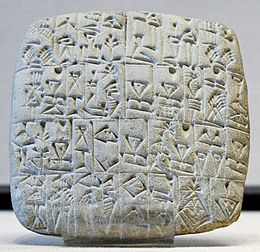
\includegraphics[width=0.4\columnwidth]{figures/sumerianSales}
    \caption{Bill of sale of a male slave and a building in Shuruppak, Sumerian tablet, circa 2600 BC}
    \label{fig:sumerianSale}
\end{figure}

Contracts are pervasive and drivers of economic change and social progress~-- it is no overstatement that civilization fundamentally relies on understanding legal documents to function.
In more than four millennia, the nature of these documents has not changed at all: they contain clauses in natural language, and we still rely on human interpretation to understand them.
In that time, the complexity of the concepts legal documents represent has increased substantially, to the point of having professions that specialise in interpreting legal documents.
This lack of change is despite the pervasiveness of contracts, their importance as drivers of economic activity, and significant technological progress.

Some technologies~(digital signing, PDF, collaborative drafting tools, etc) have changed the medium of the documents and have facilitated some hassles involved in dealing with them.
These technologies mainly target the automation of bureaucratic overheads, rather than dealing with the contents of contracts themselves and trying to reason about their contents.

Since Szabo introduced the concept of smart contracts~\cite{szabo1997smart-contracts} the benefits of technology that helps us reason about the powers and obligations contracts bring has become clear.
Such benefits include democratising understanding of legal documents, self-enforcing agreements, and having services programmatically understand their legal obligations and capabilities.
This search for new machine-readable formalisms to represent a contract is evidenced by the extensive state of the art around reasoning about legal documents.
Attempts to formalise legal agreements include smart contracts~(see~\autoref{sec:ethereum}).
While revolutionary in their capability to self-enforce agreements between parties and achieve consensus between disagreeing parties, the technology has created a new class of software systems rather than automating and disrupting the operations around existing legal documents.
Other attempts include formalisations through programming languages like The Accord Rpoject~\cite{accordHomepage} or logic calculi like Symboleo~\cite{symboleo2020}~(see~\autoref{subsec:reasoning-with-legal-agreements}).
These tend to be expressive (in that they are able to formalise a broad range of legal documents),
but are usually specified through programs or more complex specification languages or algebras.

This that means in practice they require they are specialist a strong background in engineering or logic programming to be authored and even read, which is a strong barrier to their use in industry.
They also tend to make little effort in compromising with existing frameworks for dealing with legal agreements: while being machine-readable is a desirable property of a contract, being human-readable (eg, for use in court) is a necessary property.


\section{Objectives}\label{sec:objectives}

% TODO move from evalaution
% objectives should be vague
%% should be able to express legal agreements
% expressive enough to support a large class
% natural lang rep gives you confidence it represents what you think it represents

From the above motivations we can derive the main objectives of this project.
They are motivated by how existing technologies in the state-of-the-art (see~\autoref{sec:nlp} and~\autoref{sec:machine-readable-contracts}) fail to address them, and are as follows:
\begin{itemize}
% for hi level
    \item To develop a specification language both accessible and expressive enough to represent concepts that typically make up contracts~(such as parties' obligations and powers)

    \item To develop an accessible analysis mechanism that helps parties understand their powers, obligations, and given a state of the world, understand whether they are (or how they can become) compliant with the agreement;
    as well as verifying said agreement is free of logical contradictions.

    \item To demonstrate the applicability of the developed framework in the context of legal agreements
\end{itemize}


\section{Core Contributions}\label{sec:core-contributions}
%!! change
%This project, \textbf{Confis}, is a framework that includes a specification language that allows representing a broad range of legal agreements, and a rule generation and evaluation engine that allows answering complex queries.

Please see~\autoref{fig:confis-overview} for a diagram on how these contributions interact with each other.

\subsection{A Language for Specifying Legal Agreements}
The \textbf{Confis DSL} is a domain-specific language that specifies contracts.
Like Applescript or Python, is engineered to resemble English.
It is parsimonious and formalises a small set of concepts (legal obligations, powers, and the circumstances in which they apply) in order to be simple to learn and cover a broad range of contracts.

See~\autoref{sec:language-semantics} for more details on the language.

\subsection{A Prototype Implementation of the Confis DSL}
By using Kotlin as a \emph{host language} for the DSL (see~\nameref{sec:dsls}), we present a prototype which allows compiling the Confis language.

See~\autoref{subsec:dsl-implementation} for more details on the language implementation.

\subsection{An Intelligent Editor for the Confis DSL}
By using an existing development environment, we greatly improve the accessibility of the Confis Language relative to other specification languages in the literature (like Accord or Symboleo) by also implementing a graphical prototype that eases the drafting of Confis agreements and is able to provide human-readable live previews and report errors.

See~\autoref{sec:confis-editor} for more details on the editor.

\subsection{A Querying Engine for Confis Agreements}
We also introduce a rules engine that compiles a Confis Agreement and is able to answer complex queries by generating and evaluating rules depending on the type of query.
It is able to answer queries relating to determining the legal capabilities of parties, finding contradictions in an agreement, determining clause violations depending on past events, and determining necessary steps towards compliance.
To better illustrate the extent of the querying, some questions that can be executed as queries are:
\begin{itemize}
    \item \emph{`Under what circumstances can my landlord evict me?'}
    \item \emph{`I have paid my rent late -- am I in breach of the contract?'}
    \item \emph{`What do I need to do to in order to be fully compliant?'}
    \item \emph{`Am I allowed to derive statistics from this licensed dataset with commercial purposes?'}
\end{itemize}
In contrast with the state of the art, the solution is self-contained and does not require the user to translate a Confis specification into other formalisms.

See~\autoref{sec:rule-generation} for more details on the querying engine.

% make subsecs for contribs

\subsection{A User Interface for Querying Documents}
In addition to the formalisms necessary to examine a contract by querying it, we introduce a prototype that allows asking these questions through an accessible graphical user interface, and producing understandable human-readable answers to them.

See~\autoref{sec:queryUI} for more details on the querying UI\@.


% beauty is ver short distance from having written to answering sphisticated queries

% no need for further translation and somehow efficient


\section{Project Overview}\label{sec:project-overview}

This section hopes to provide a more concrete high-level overview of how the core contributions together form the Confis framework, which combines the different user interfaces, the editor, and the human-readable preview.
A screenshot depicting the user interfaces can be found in~\autoref{fig:geophys-full-editor}.

An architectural diagram of how all components interact with each other in~\autoref{fig:confis-overview}.

\begin{figure}[h]
    \centering
    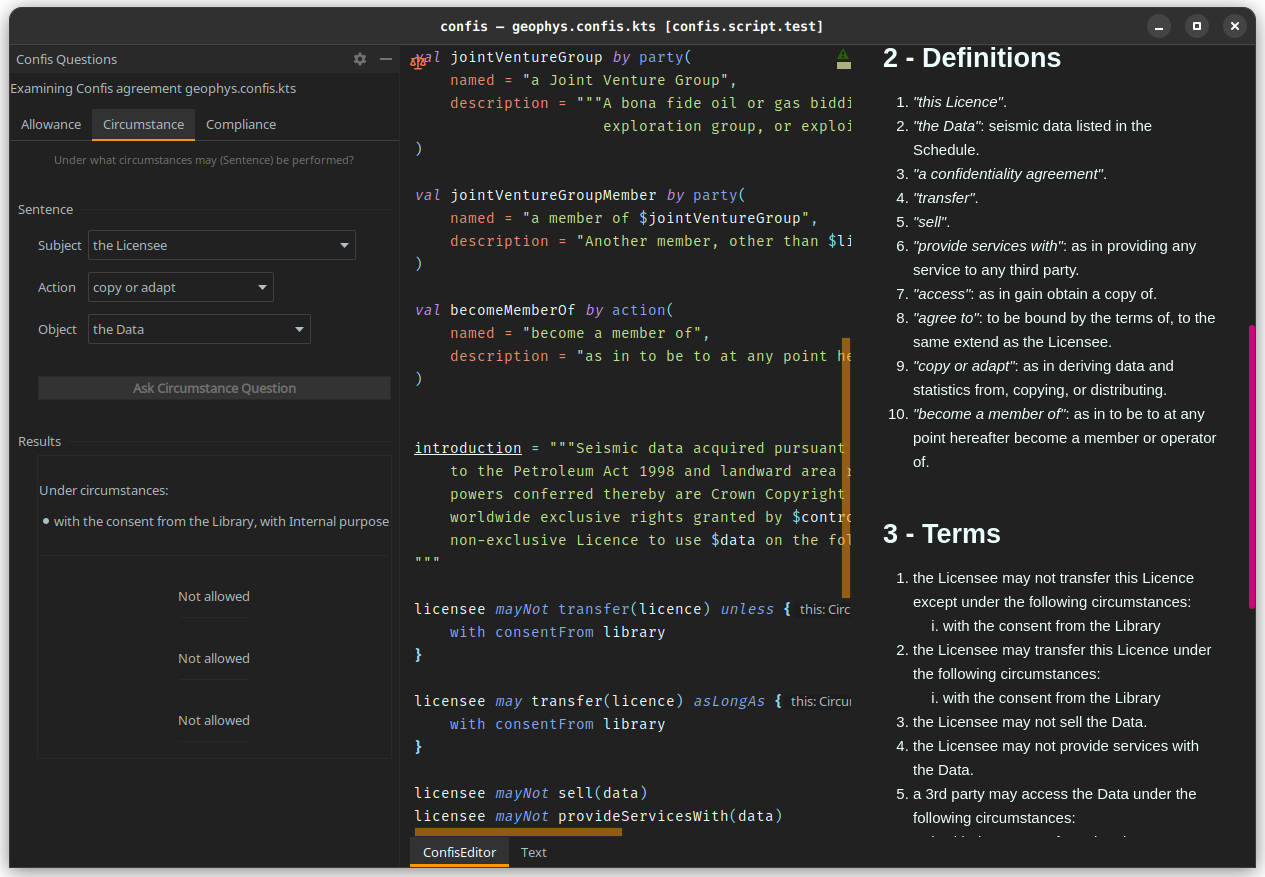
\includegraphics[width=\columnwidth]{figures/confis.full-geophys}
    \caption
    [Screenshot of the Confis Editor and Query UI]
    {Screenshot of the Confis Editor and Query UI, depicting a Confis version of a license for seismic data~\cite{seismicDataLicence}
    \par\footnotesize

    From left to right: the \textbf{Query UI} that allows querying the agreement; the \textbf{Confis code} specifying the agreement; a \textbf{live preview} of the agreement in generated English text.
    }
    \label{fig:geophys-full-editor}
\end{figure}

Aside from this introduction and the background research~(\autoref{ch:background}), the main body of this report is divided in two parts: \autoref{ch:lang}, covering the Confis language, and~\autoref{ch:queries}, covering the querying of documents specified in said language.
Both chapter discuss the requirements, design, tooling, and implementation of each part.

\tikzset{font={\fontsize{9pt}{10}\selectfont}}
\begin{figure}[h]
    \usetikzlibrary{shapes.misc, arrows.meta}
    \colorlet{pastelBlue}{blue!40!white}

    \begin{tikzpicture}
        [
        node distance=2cm and 1.8cm,
        >={Stealth[inset=0pt,length=7pt,angle'=30,round]},
        ]
        \node (user) [
            rectangle,
            rounded corners,
            text=white,
            fill=mdtBlue,
        ] {\textbf{Contract Drafter}};

        \node (docs) [
            draw,
            align=left,
            rectangle,
            rounded corners,
            above=of user,
            rectangle,
        ] {
            \textbf{Online Documentation}\\
            \emph{Uses:}\\HTML pages generated\\from Markdown\\
            \emph{See:}\\\nameref{sec:language-documentation}
        };

        \node (editor) [
            draw,
            text width=3cm,
            rectangle,
            rounded corners,
            below=of user,
            rectangle,
        ] {
            \textbf{Confis Editor}\\
            \emph{Uses:}\\IntelliJ IDEA\\
            \emph{See:}\\\nameref{sec:confis-editor}
        };

        \node (lang) [
            draw,
            rectangle,
            rounded corners,
            text width=4cm,
            left=of editor,
        ] {
            \textbf{Confis Language}\\
            \emph{Uses:}\\Kotlin as host language for DSL\\
            \emph{See:}\\\nameref{sec:language-semantics}
        };

        \node (queryUi) [
            draw,
            text width=3cm,
            rectangle,
            rounded corners,
            right=of editor,
        ] {
            \textbf{Query UI}\\
            \emph{Uses:}\\IntelliJ IDEA\\
            \emph{See:}\\\nameref{sec:queryUI}
        };

        \node (compiler) [
            draw,
            text width=3cm,
            rectangle,
            rounded corners,
            below=of editor,
        ] {
            \textbf{Compiler}\\
            \emph{Uses:}\\Kotlin Compiler\\
            \emph{See:}\\\nameref{subsec:dsl-implementation}
        };

        \node (queryEngine) [
            draw,
            text width=3cm,
            rectangle,
            rounded corners,
            right=of compiler,
        ] {
            \textbf{Query Engine}\\
            \emph{Uses:}\\EasyRules\\
            \emph{See:}\\\nameref{sec:rule-generation}
        };

        \draw[->]
        (user.west)
        to [out=180,in=90]
        node [yshift=0.7cm, text width=6cm]{Formalises agreement into Confis\\semantics as text}
        (lang);

        \draw[->] (lang.east)
        -- node [above, align=center] {Written\\into}
        (editor);

        \draw[->] (editor.270-15)
        -- node[left] { Compiles text }
        (compiler.90+15);

        \draw[->]
        (compiler.90-15)
        -- node[right, text width=3cm] { Compiler\\feedback\\and IR}
        (editor.270+15);

        \draw[->] (editor.north)
        -- node[align=center, fill=white] { Visual feedback }
        (user);

        \draw[->] (editor.east)
        -- node[above, align=center] { Broadcasts\\IR }
        (queryUi);

        \draw[->] (queryUi.270-15)
        -- node[left, text width=2cm, align=right] { IR and\\compiled\\query }
        (queryEngine.90+11);

        \draw[->]
        (queryEngine.90-11)
        -- node[right, text width=3cm] { Query\\result }
        (queryUi.270+15);

        \draw[->]
        (docs.south)
        -- node[align=center, fill=white] { Provides knowledge\\ \& examples }
        (user);

        \draw[->]
        (queryUi.90-15)
        to [out=90,in=10]
        node [above, yshift=0.2cm, fill=white, align=left]{Query rendered\\as English text}
        (user);

        \draw[->]
        (user)
        to [out=-10,in=90]
        node [below, yshift=0.6cm, xshift=-0.8cm, fill=white, align=center]{Query\\selection}
        (queryUi.90+15);

    \end{tikzpicture}
    \caption{Overview of the different components of Confis}
    \label{fig:confis-overview}
\end{figure}
